\chapter{Exploration of Visualization Techniques through Survey} \label{chap:explor}
In the previous chapter we studied existing interaction techniques combining AR, feedforward and ubicomp. We will now perform our own exploratory study of the design space. Through an online survey with 34 participants, we test seven visualizations for showing which lights are connected to which switches. The most promising of these visualizations receive a more high-fidelity implementation in the next chapter. See Appendix \ref{chap:explor_survey} for a full printout of the survey.

\section{Procedure} \label{sec:explor:procedure}
We start by collecting the gender and age of each participant, to have a general idea of our demographics. Next, we want to have the participants try out a set of scenarios and to rate them on various aspects. Each of these scenarios will have some problem that the participants must try to solve. Some will be baseline scenarios where the participants receive no help, but most will be augmented scenarios where the participants are aided in their task by some form of AR feedforward that we wish to evaluate.

Since our survey targets the general population, AR and ubicomp may be foreign concepts to some participants, and thus we must take special care not to confuse or overwhelm them. We also prefer the setups to offer problems that the participants have encountered before, helping them to understand the task and stimulating them. For this reason, we opted to focus on the problem of matching light switches with their corresponding lights. This is a recognizable and conceptually simple problem, but still allows for some complexity in the setups. We also know from Section \ref{sec:relat:previewable_switch} that feedforward can indeed be a valuable tool in solving this problem \cite{park2014previewable}.

Our next question is how many and which setups to choose. Ideally, we would use only one setup for all scenarios, to eliminate an extra variable from our experiment. A second reason to limit the number of setups is that for each setup we must add a baseline scenario without feedforward to compare the other scenarios against. However, the set of possible setups is extremely diverse. A symmetric rectangular hall with a grid of lights on the ceiling might benefit most from different approaches than a cozy lounge with various lights on walls and tables. We could test each approach in multiple setups, but this would reduce the number of approaches we could include.

We decide on using two setups, which limits the number of baselines, but still allows for some variety in the scenarios. We will test each feedforward approach only in the setup in which we expect it to work best, to maximize the number of approaches that we can investigate. This choice reflects the explorative nature of this study. The promising approaches can still be investigated further in a follow-up study. Both of the chosen setups are of moderate complexity, to create scenarios that challenge our approaches but that one might still encounter in day-to-day life.

The first setup is the \textit{classroom}, shown in Figure \ref{fig:explor:classroom_baseline}. It is a highly symmetric setup comprised of a rectangular room with a 3x3 grid of lights on the ceiling and a row of 3 switches, one large and two small, next to the door. This is a real room from around our workplace, and its unintuitive arrangement of the light switches, described in the image annotation, helped spark our interest in its matching problem. We intend this to be the simpler of our two setups, because we believe it has a straightforward solution (which is sadly not used in the actual room), being that every switch controls the row of lights closest to it. However, some confusion may be introduced by the facts that one switch is larger than the others, and that the spacing between the rows of lights is unequal.
    
\begin{figure}
    \centering
    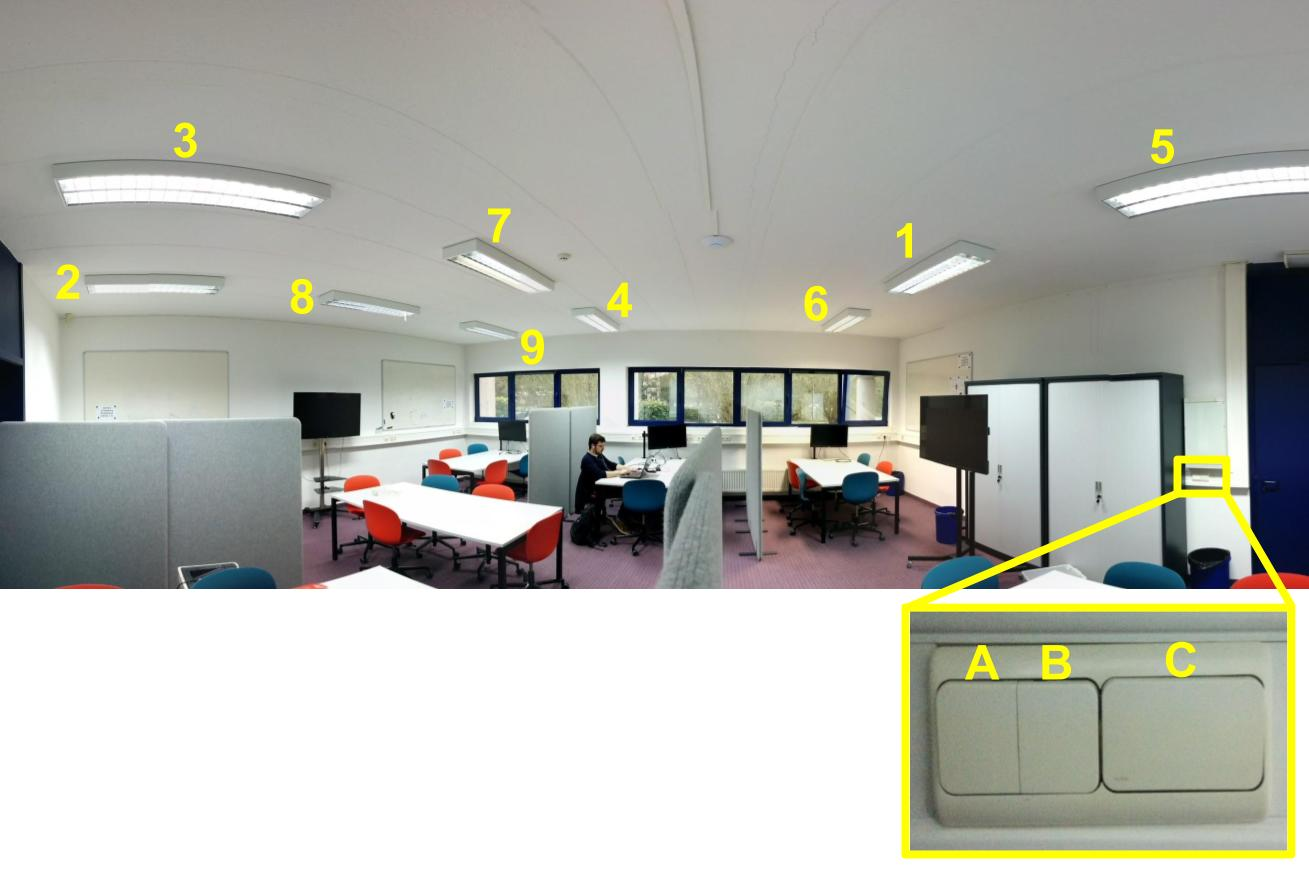
\includegraphics[width=0.8\linewidth]{exploration/classroom_baseline.jpg}
    \caption{The \textit{classroom} scenario, containing a 3x3 grid of lights and a row of three switches. Survey participants are asked how they believe the lights are connected in this room. The lights are numbered randomly so as to not influence the responses. The actual configuration is rather unintuitive: switch A controls lights 2, 3 and 5, switch B controls lights 9, 4 and 6, and switch C controls lights 8, 7 and 1.}
    \label{fig:explor:classroom_baseline}
\end{figure}

Our second setup is the \textit{kitchen}, shown in Figure \ref{fig:explor:kitchen_baseline}. We have taken this picture from Wikimedia Commons \cite{FileTROY82:online} and so we do not know how its lights might be connected. We have chosen this room for its variety of wall, hanging and ceiling lights, six in total. There are four light switches, one larger than the rest, arranged in two rows. This setup is meant to be the more complex of the two. We chose it because we believe there is no single obvious mapping of switches on lights. We might create matches based on similar locations, sizes, or some other metric, but in many cases these metrics will contradict each other. This conflict is intentional, as it allows us to determine which metrics the participants will choose over others.

\begin{figure}
    \centering
    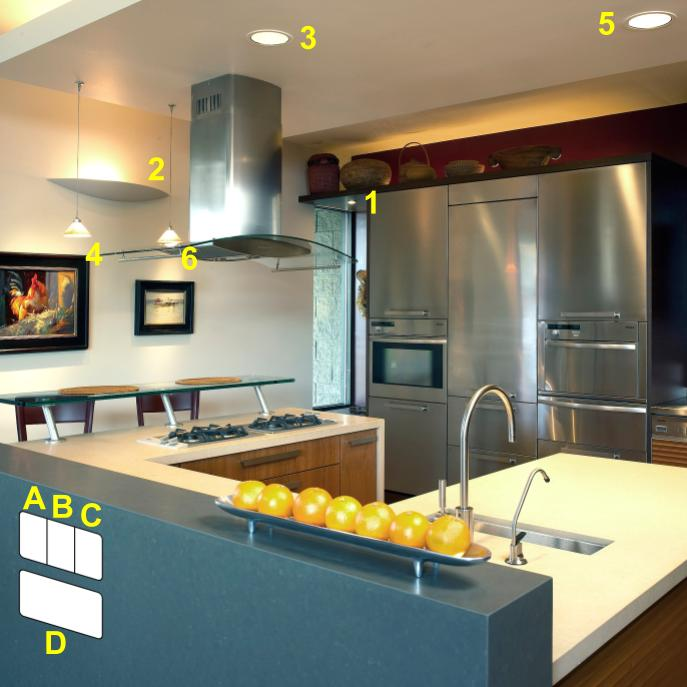
\includegraphics[width=0.8\linewidth]{exploration/kitchen_baseline.jpg}
    \caption{The \textit{kitchen} scenario, with a variety of lights in different locations and four switches arranged in two rows. Survey participants are asked how they believe the lights are connected in this room. The lights are numbered randomly so as to not influence the responses. The actual configuration is unknown to us.}
    \label{fig:explor:kitchen_baseline}
\end{figure}

After a short introduction and collection of demographics, as mentioned before, the first scenario we present participants with is the kitchen baseline scenario, meaning a picture of the room as shown in \ref{fig:explor:kitchen_baseline}, without any visualizations for aid. Participants are explained that ``Each image will have some yellow annotations on it, which are not part of the image and are only present to simplify the answering process; when thinking about the questions, you should act like the yellow annotations do not exist''. Then, participants are asked ``According to you, which switches control which lights, based on this image?'' and receive a grid to mark their answers. Next, they are asked ``How certain are you that the switches work the way you indicated?'' on a 1-5 Likert scale. Finally, we ask ``What role did the following assumptions play when you solved this scenario?'' and give them seven assumptions:
\begin{itemize}
    \item Each switch controls the lights that are closest to it.
    \item Higher placed switches control larger lights.
    \item Higher placed switches control more lights.
    \item Larger switches control larger lights.
    \item Larger switches control more lights.
    \item Larger switches control lights that are closer to it.
    \item Larger switches control lights that are further away from it.
\end{itemize}
For each assumption, participants must choose between ``no role'', ``small role'' and ``large role''. We also provide a text field for any other assumptions or general remarks that participants might want to add.

After the baseline kitchen scenario comes the baseline classroom scenario. Both work exactly the same, with the same questions, just different rooms. The purpose of both baseline scenarios is of course to get some insight into how people reason about the matching of lights and switches, and into what they consider logical arrangements. Knowing how people reason and what assumptions people will make intuitively, might allow us to design better visualization by building upon those same principles.

After the two baseline scenarios follow seven augmented scenarios, which make up the main part of our survey.  First, participants receive a short introduction to AR, which uses Pokémon Go as an example. Then, they are told ``For the remainder of the survey, imagine you are looking at the world through a smartphone or through an augmented reality headset. In each of the following scenarios, your AR device will try to aid you by augmenting your vision in some way. Anything yellow is not part of these visualizations''.

For each of the seven augmented scenarios, the participant is asked to match the switches and the lights in an answering grid, in the way they believe is indicated by the visualization. Next, we ask them once more how certain they are of their answer, on a 1-5 Likert scale. Then comes a new question: ``I believe that, in real life, the above visualization would be...'':
\begin{itemize}
    \item Easy to learn
    \item Fast to work with
    \item Resistant to errors
    \item Useful
    \item Enjoyable
\end{itemize}
Participants again have to answer on a 1-5 Likert scale for each of these five dimensions, which are derived from five of the Nielsen heuristics for user interface design \cite{nielsen1990heuristic}. They give us an indication of how the participants perceive each of the visualizations, and the perceived resistance to errors might be interesting to compare to the actual correctness of the participant's matching grids.

The first visualization we present to the participants is the \textit{colors} visualization, which matches lights and switches by marking them with dots of the same color, as shown in Figure \ref{fig:explor:colors_vis}. We expect this to be a very intuitive and effective visualization, and we placed it first in the hopes of gradually easing the participants into their task. To illustrate how natural the visualization is, this is the technique we used without thinking to mark the circuits in our own notes, and other people could understand them without giving them a second glance. We are interested to see if we can find visualizations that outperform colors, maybe even just in specific cases, which is why we included it for comparison.

\begin{figure}
    \centering
    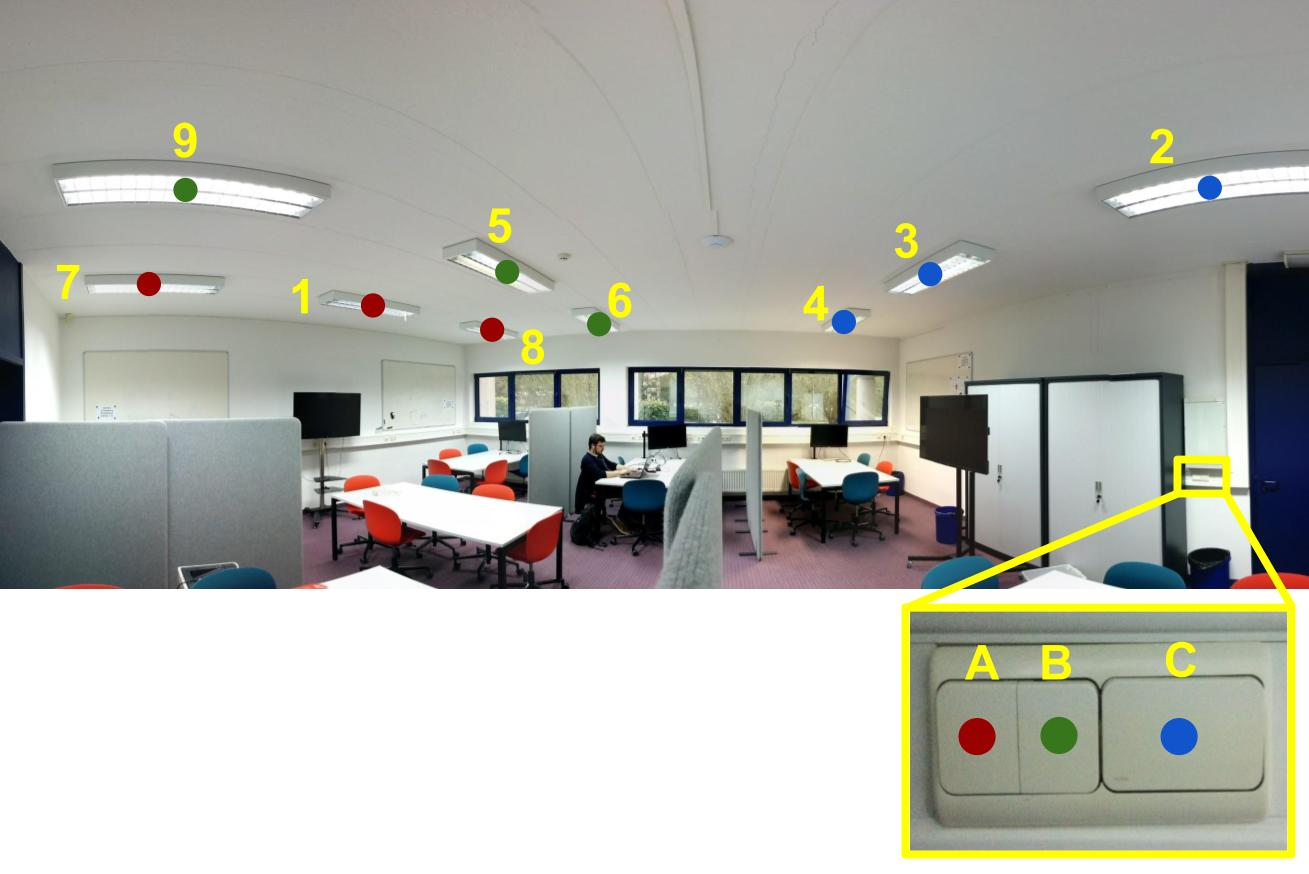
\includegraphics[width=0.8\linewidth]{exploration/colors.jpg}
    \caption{The \textit{colors} visualization, matching lights and switches by marking them with dots of the same color.}
    \label{fig:explor:colors_vis}
\end{figure}

The second visualization we call \textit{shapes}, shown in Figure \ref{fig:explor:shapes_vis}, and it matches lights and switches by marking them with the same shapes. It is again a straightforward visualization, much like numbering the circuits would be, although we expect this visualization will be slightly less popular than the colors, because we feel that repeatedly recognizing shapes requires some mental effort that colors do not. However, both visualizations share a weakness that may not be immediately apparent from these static images: when the user looks away from the lights, they have no indication of where or even how many lights are connected. The user must still find and count all lights themselves, and they have no easy way to make sure they have not missed any. Our next visualizations will attempt to mitigate this issue.

\begin{figure}
    \centering
    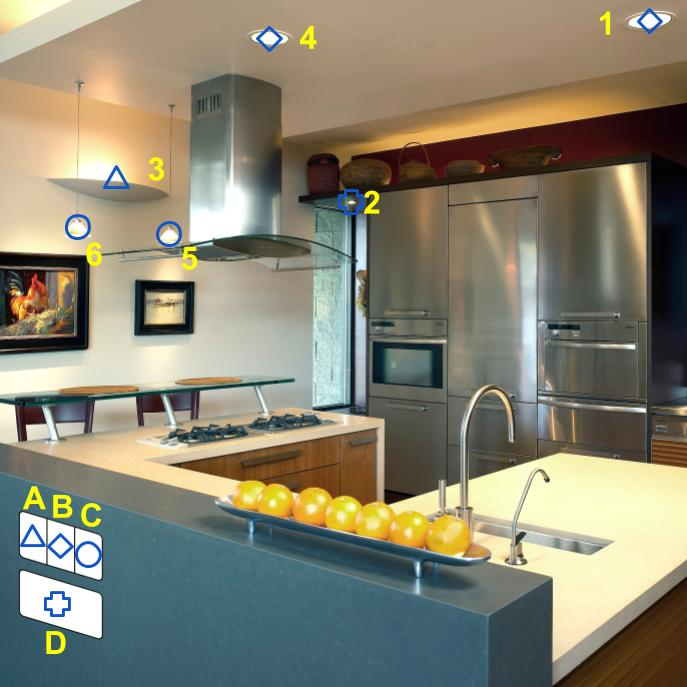
\includegraphics[width=0.8\linewidth]{exploration/shapes.jpg}
    \caption{The \textit{shapes} visualization, matching lights and switches by marking them with the same shapes.}
    \label{fig:explor:shapes_vis}
\end{figure}

Our third visualization is the \textit{minimap}, shown in Figure \ref{fig:explor:floor_plan_vis}, which displays only one circuit at a time. The switch belonging to the active circuit is highlighted, and a minimap of the room, shown somewhere in the user's vision, highlights the corresponding lights. This way, the user always has an overview of how many and which lights are connected, no matter where their gaze is oriented. A user who is familiar with the room might even be able to locate the lights without looking at them, just by recognizing their locations on the minimap, and a user who is not familiar with the room might still deduce which directions to search in.

\begin{figure}
    \centering
    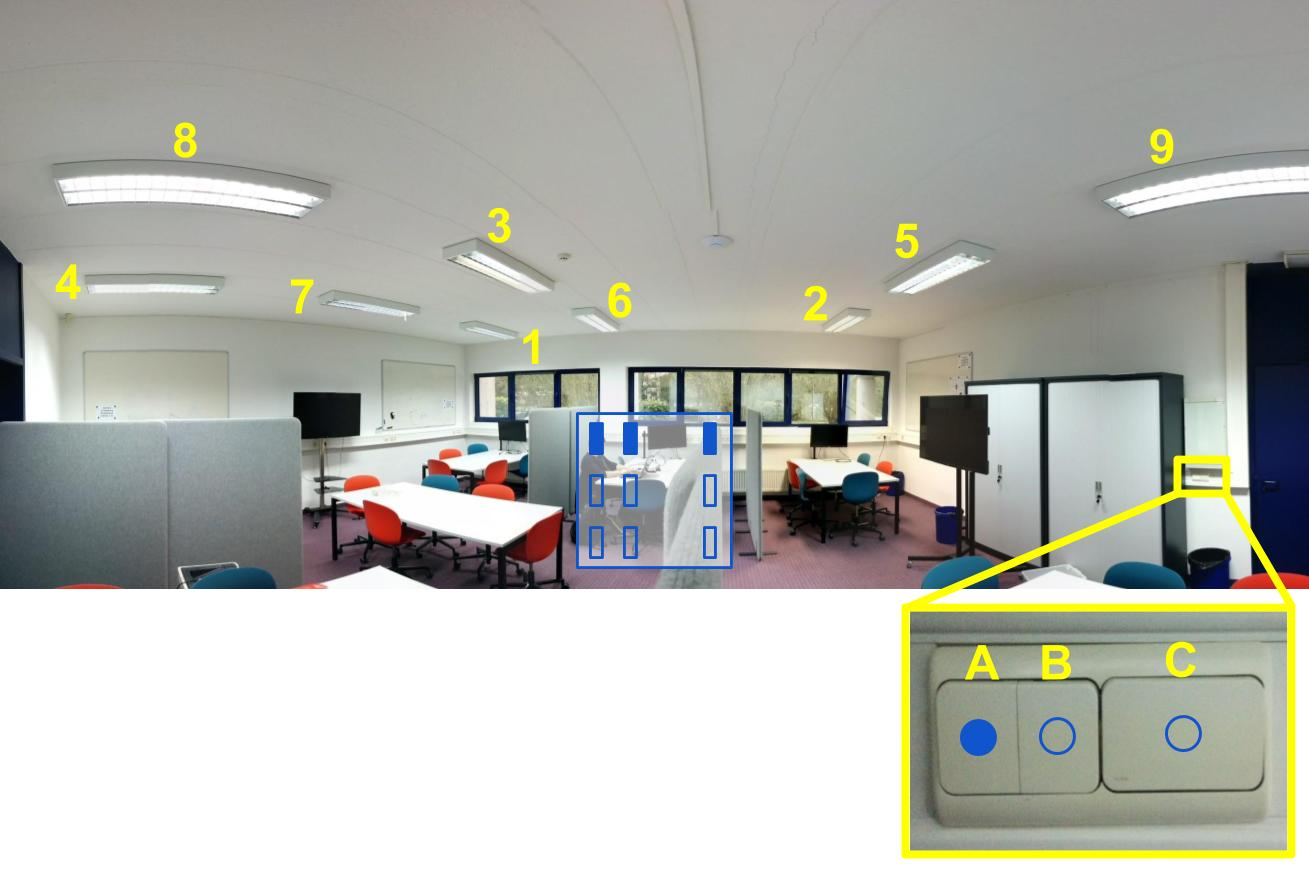
\includegraphics[width=0.8\linewidth]{exploration/floor_plan.jpg}
    \caption{The \textit{minimap} visualization, matching lights and switches by displaying a minimap somewhere in the user's vision, on which all lights are displayed, and then one by one highlighting a single switch and its corresponding lights on the minimap.}
    \label{fig:explor:floor_plan_vis}
\end{figure}

The fourth visualization we call \textit{switches on lights}, and it is shown in Figure \ref{fig:explor:switches_on_lights_vis}. On each light, an image of the entire switch panel is shown, and the connected switch is highlighted. Logically, we expect this visualization to be useful for quickly finding a light's connected switch, however, for the other way around, all lights still have to be searched. We also suspect this visualization does not allow for quick glancing to distinguish the different circuits, as the different highlights are not so visually distinct.

\begin{figure}
    \centering
    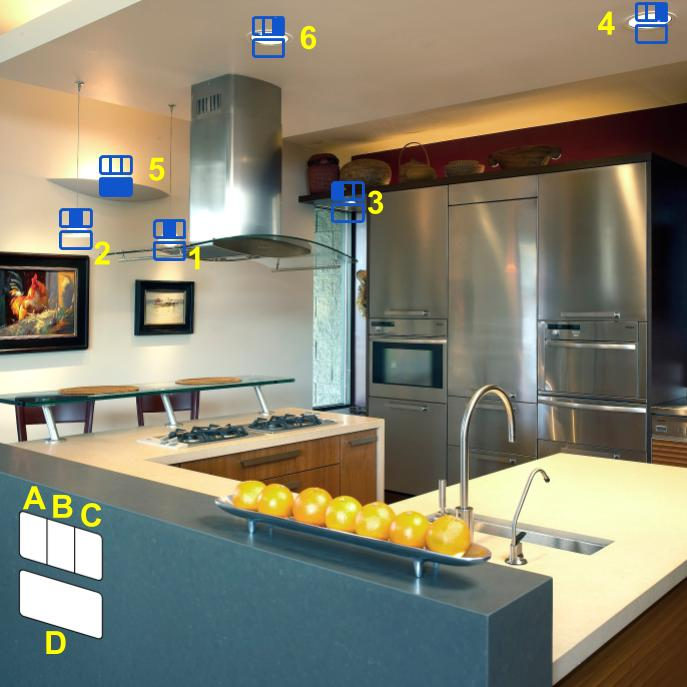
\includegraphics[width=0.8\linewidth]{exploration/switches_on_lights.jpg}
    \caption{The \textit{colors} visualization, matching lights and switches by showing an image of the switches on each light, with the connected switch highlighted.}
    \label{fig:explor:switches_on_lights_vis}
\end{figure}

Our fifth visualization, the \textit{lights on switches}, shown in Figure \ref{fig:explor:lights_on_switches_vis}, is the opposite of the previous one, as the name suggests. On each switch, a floor plan is shown on which the connected lights are highlighted. Correspondingly, we assume this is an effective visualization for quickly finding a switch's connected lights, but less so the other way around. In contrast to the previous visualization, we expect this one to be ideal for quickly getting an overview of the general layout of the circuits, as each circuit is neatly displayed on its corresponding switch.

\begin{figure}
    \centering
    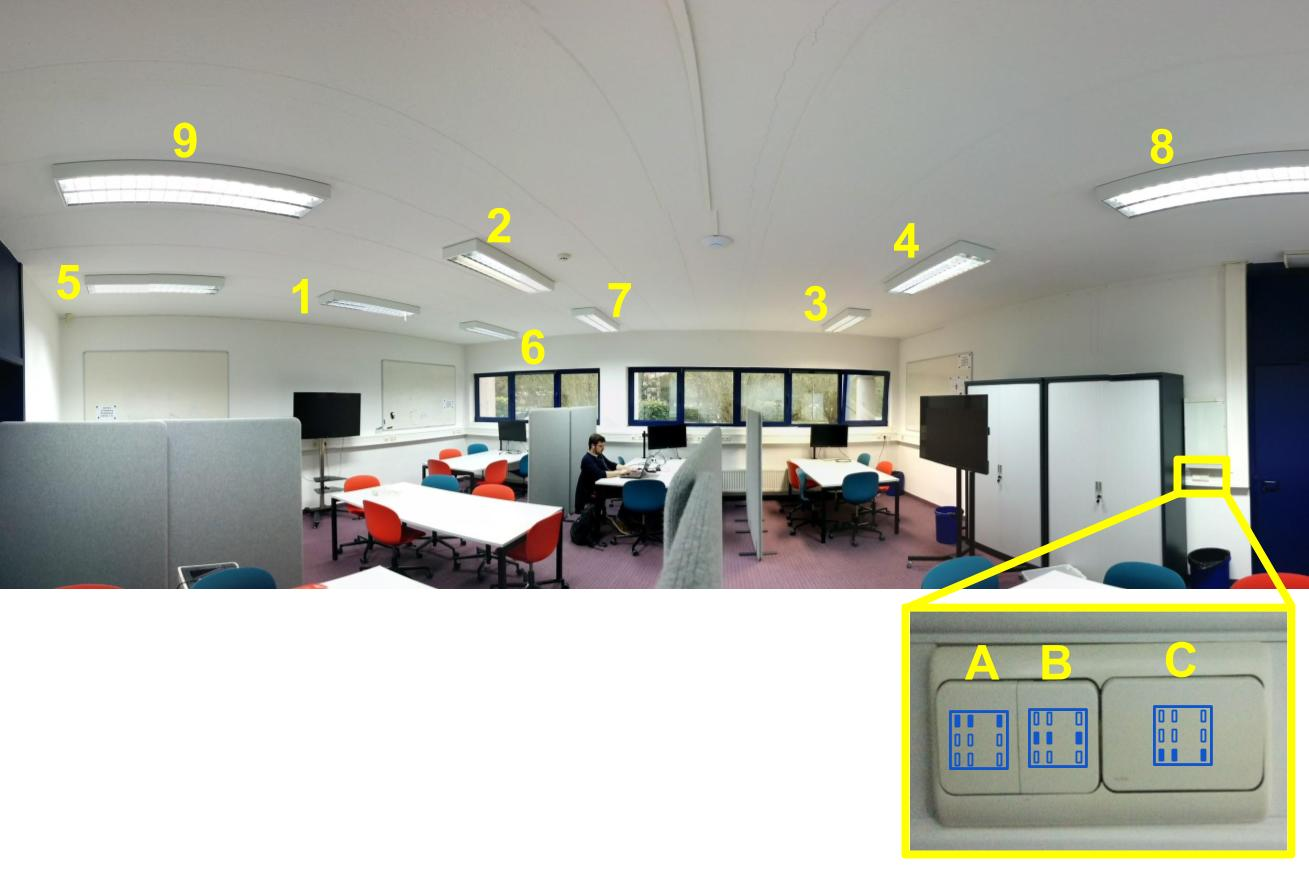
\includegraphics[width=0.8\linewidth]{exploration/lights_on_switches.jpg}
    \caption{The \textit{lights on switches} visualization, matching lights and switches by showing a floor plan on each switch, with the connected lights highlighted.}
    \label{fig:explor:lights_on_switches_vis}
\end{figure}

We started with two visualizations that do not improve spatial understanding, and followed up with three visualizations that help in a roundabout way. The use of minimaps or abstract views provides an indirect mapping that requires a translation step from the user, who has to relate these views to the real world. Direct mappings are also possible, and we are interested to see how they compare with the previous approaches. Therefore, our last two visualizations are directional indicator, which point the user's gaze directly towards the point of interest. The first is called \textit{lines}, shown in Figure \ref{fig:explor:lines_vis}, and it draws straight lines between each switch and its corresponding lights. To increase contrast, each circuit's lines have their own dotted pattern. In this visualization, no translation step is required from the user, as they simply have to follow the lines, and they can even do so in both directions.

\begin{figure}
    \centering
    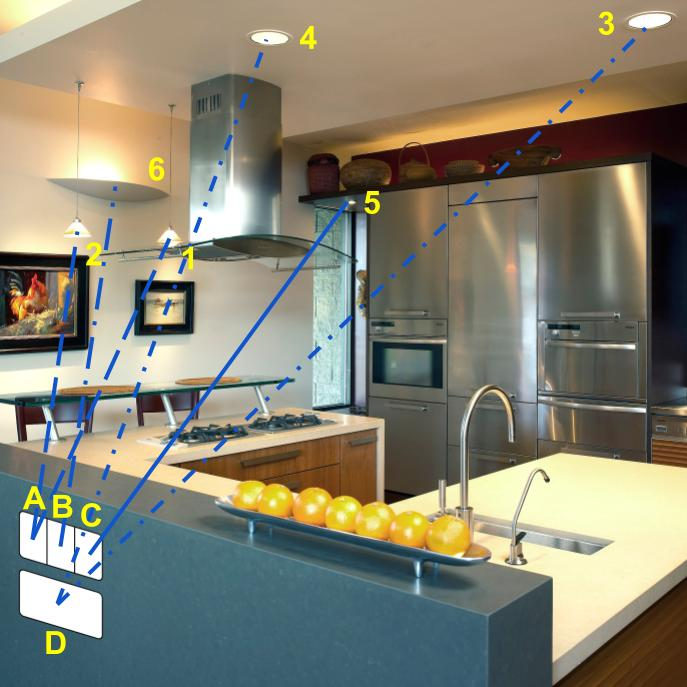
\includegraphics[width=0.8\linewidth]{exploration/lines.jpg}
    \caption{The \textit{lines} visualization, which shows a straight line running between the switches and each of their lights. Each circuit has a different line pattern for contrast.}
    \label{fig:explor:lines_vis}
\end{figure}

The second directional indicators, and the last of our visualization, are the \textit{arcs}. They are pointed semi-circles around the switches pointing at their corresponding lights, as shown in Figure \ref{fig:explor:arcs_vis}. Such pointers are already commonly used in 3D shooter games to show the player from which direction they are being shot. We wish to investigate how well this approach translates to AR and to other use cases.

\begin{figure}
    \centering
    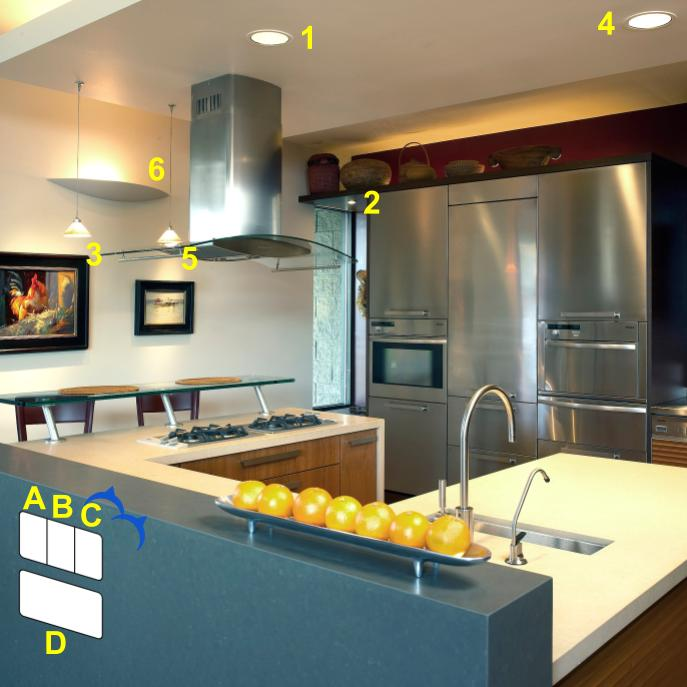
\includegraphics[width=0.8\linewidth]{exploration/arcs.jpg}
    \caption{The \textit{arcs} visualization, which shows pointed semi-circles around each switch pointing at its corresponding lights.}
    \label{fig:explor:arcs_vis}
\end{figure}

We concluded our survey with several questions about dimmers. We did not test any visualizations, but rather we investigated which type of dimmer the participants prefer, and which actions they find natural for achieving specific goals. We thought this knowledge might prove useful for our high-fidelity implementation, and since it made the survey only slightly longer, we considered it a worthwhile addition.

First, we showed participants the leftmost switch in Figure \ref{fig:explor:switches}, which we called the \textit{standard switch}, and we gave them three possible actions: short press, long press and double press. We also gave two goals: increase the brightness of the lights and turn off the lights. For each combination of an action and a goal, six in total, participants had to answer on a 1-5 Likert scale how intuitive they found this action to achieve this goal. Next, we repeated these questions for the middle switch in Figure \ref{fig:explor:switches}, called the \textit{rotating switch}, for which we gave participants two extra actions: rotate clockwise and rotate counterclockwise. Finally, we asked the participants which switch they would prefer to control the brightness of a light, when given the choice between a rotating switch and a \textit{sliding switch}, shown on the right in Figure \ref{fig:explor:switches}. Participants could also answer ``I have no preference'', ``I don't know'' or describe a custom choice.

\begin{figure}
    \centering
    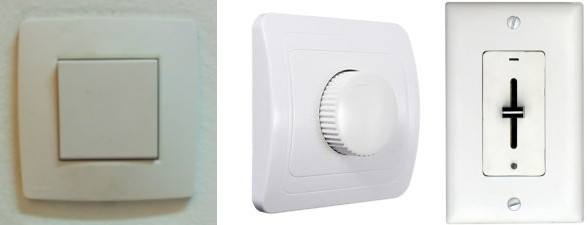
\includegraphics[width=1.0\linewidth]{exploration/switches.jpg}
    \caption{...}
    \label{fig:explor:switches}
\end{figure}

\section{Apparatus} \label{sec:explor:apparatus}
The survey was created and hosted using Google Forms. It was made available via several online media for the duration of one week, from 2017-11-08 until 2017-11-15. We estimate the average completion time at 20 minutes.

\section{Participants} \label{subsec:explor:participants}
The survey received a total of 36 unpaid responses. After careful consideration, we chose to discard two responses. In the first discarded submission, the participant wrote that they could not answer some questions due to technical difficulties, and in the second, the participant's commentary clearly showed that they had misunderstood some questions. Our results and analysis are thus based on 34 responses, with demographics as shown in Table \ref{table:explor:demographics}. The average age of the participants was 27 years.

    \begin{table}
    \centering
        \begin{tabular}{|c|c c|c|} 
        \hline
                  & Male & Female &    \\
        \hline
        Age 17-25 &   18 &      8 & 26 \\
        Age 33-53 &    5 &      3 &  8 \\
        \hline
                  &   23 &     11 & 34 \\
        \hline
        \end{tabular}
    \caption{Demographics}
    \label{table:explor:demographics}
    \end{table}

\section{Results \& Discussion} \label{sec:explor:res_disc}
%We start off by discussing the two baseline scenarios. The first question we wanted to ask ourselves after closing the survey was ``What is the most common solution for each scenario, and how common is it?''. In other words, we want to know whether a consensus is reached, or if there is total disagreement among respondents. Figures \ref{fig:preliminary_study_kitchen_baseline_consensus} and \ref{fig:preliminary_study_classroom_baseline_consensus} show the most common solution for both baseline scenarios, by putting the labels of connected lights and switches in the same color. The consensuses are also summarized in table \ref{table:preliminary_study_consensus}.

\clearpage

\begin{table}
    \centering
    \begin{tabular}{|c|c|c|c|} 
    \hline
    A     & B       & C                     & Times given \\
    \hline
    2 8 9 & 3 4 7       & 1 5 6             & 21     \\
    1 5 6 & 2 3 4 7 8 9 & 1 2 3 4 5 6 7 8 9 &  3     \\
    1 5 6 & 3 4 7       & 2 8 9             &  2     \\
          &             & 1 2 3 4 5 6 7 8 9 &  2     \\
    4 6 9 & 1 7 8       & 2 3 5             &  1     \\
    3 4 7 & 1 5 6 8     & 2 9               &  1     \\
    2 3 5 & 4 6 9       & 1 7 8             &  1     \\
    4 6 9 & 2 3 5       & 1 7 8             &  1     \\
    2 3 5 & 1 8 9       & 4 6 9             &  1     \\
    1 5 6 & 2 3 4 7 8 9 &                   &  1     \\
    \hline
    2 3 5 & 4 6 9       & 1 7 8             &  0     \\
    \hline
\end{tabular}
\caption{All proposed solutions for the \textit{classroom} scenario, along with the number of times they were given. The last line is the actual configuration, which was given by no one.}
\label{table:classroom_answers}
\end{table}

\begin{figure}
    \centering
    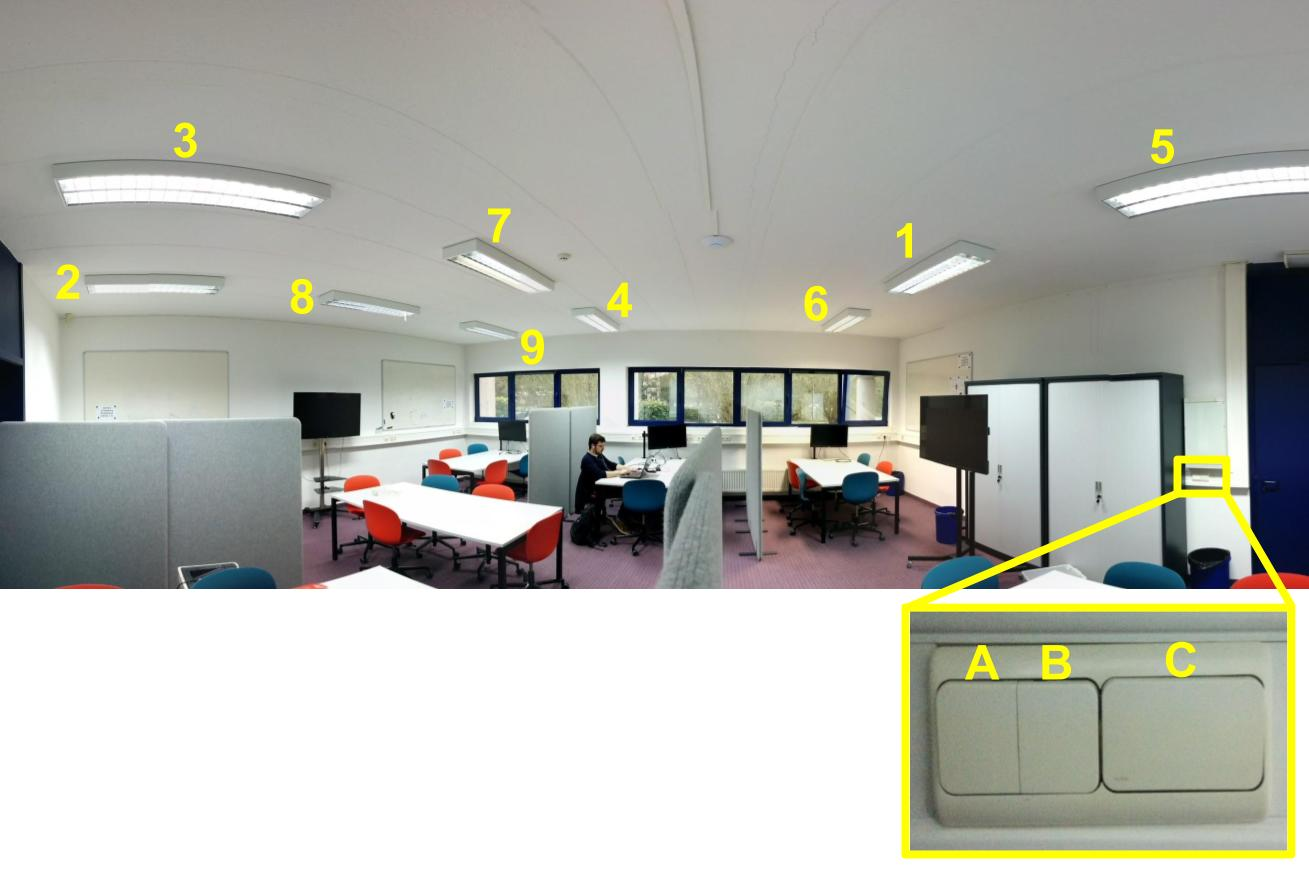
\includegraphics[width=0.8\linewidth]{exploration/classroom_baseline.jpg}
    \caption{The \textit{classroom} baseline scenario.}
    \label{fig:explor:classroom_baseline_again}
\end{figure}

\clearpage

\begin{table}
    \centering
    \begin{tabular}{|c|c|c|c|c|} 
    \hline
    A     & B   & C   & D             & Times given \\
    \hline
    2     & 4 6   & 1   & 3 5         & 9 \\
    4 6   & 2     & 1   & 3 5         & 4 \\
    1 2   & 4 6   & 3 5 &             & 2 \\
    1     & 4 6   & 3 5 & 2           & 2 \\
    1 2 4 & 4     & 2 5 & 1 6         & 1 \\
    6     & 1     & 2   & 3 4 5       & 1 \\
    4 6   & 3 5   & 1 2 &             & 1 \\
    2     & 1 3 5 & 4 6 & 1 2 3 4 5 6 & 1 \\
    2     & 1     & 4 6 & 3 5         & 1 \\
    1 2   & 4 6   & 3 5 & 3 4 5 6     & 1 \\
    4 6   & 1     & 3 5 & 2           & 1 \\
    2     & 4 6   & 3 5 & 1           & 1 \\
    2     & 4 6   & 5   & 1 3         & 1 \\
    4 6   & 1     & 2   & 3 5         & 1 \\
    2 4 6 & 1     & 5   & 3           & 1 \\
    2 3 4 & 2     & 6   & 1           & 1 \\
    1 2   & 4 6   & 3 5 & 6           & 1 \\
    4 6   &       &     & 1 2 3 5     & 1 \\
    4 6   & 1     & 3 5 & 2           & 1 \\
    3 5   & 4 6   & 2   & 1           & 1 \\
    2 5   & 2     & 1   & 4 6         & 1 \\
    \hline
\end{tabular}
\caption{All proposed solutions for the \textit{kitchen} scenario, along with the number of times they were given.}
\label{table:kitchen_answers}
\end{table}

\begin{figure}
    \centering
    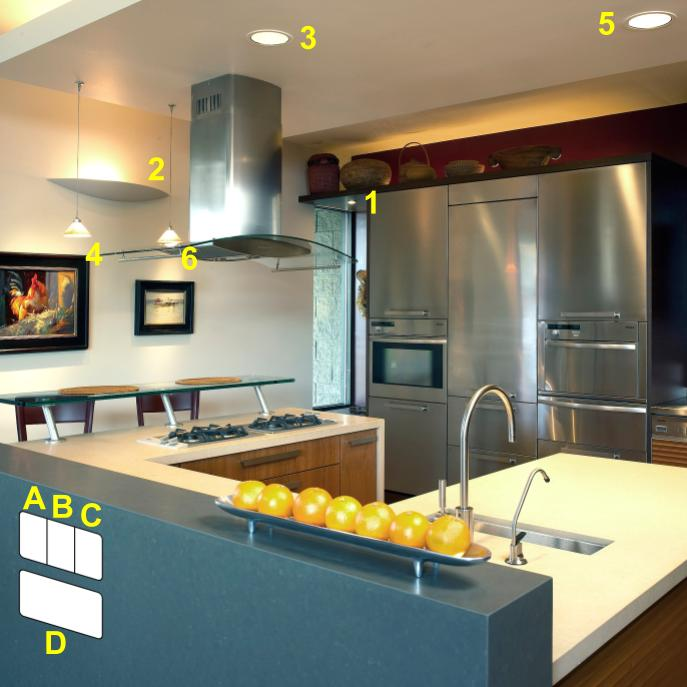
\includegraphics[width=0.6\linewidth]{exploration/kitchen_baseline.jpg}
    \caption{The \textit{kitchen} baseline scenario.}
    \label{fig:explor:kitchen_baseline_again}
\end{figure}

\clearpage

\begin{table}
    \centering
    \begin{tabular}{|c|c|c|} 
    \hline
      & Kitchen & Classroom \\
    \hline
    A & 2       & 2, 8, 9   \\
    B & 4, 6    & 3, 7, 4   \\
    C & 1       & 1, 5, 6   \\
    D & 3, 5    & N/A       \\
    \hline
\end{tabular}
\caption{Baseline scenario consensuses}
\label{table:preliminary_study_consensus}
\end{table}

For the kitchen scenario, the most common solution was given by 10 out of 34 respondents, or 29.41\%. In total, 20 different solutions were offered. We believe this shows strong disagreement, since no configuration would be intuitive for even a third of the respondents. For the classroom scenario, the most common solution was given by 21 out of 34 respondents, or 61.76\%. In total, 9 different solutions were offered. We believe this shows a clear consensus, but is still problematic because no matter the configuration, at least one in three respondents would find it confusing.

%Next we wanted to know the rationale behind the given solutions. In the survey, seven assumptions were provided, and for each of them, the respondent had to indicate whether it played ``no role'', a ``small role'' or a ``large role'' in determining their solution. The results can be seen in Figure \ref{fig:preliminary_study_rationales}. In this bar chart, we awarded one point to an assumption each time a respondent indicated it played a ``large role'', half a point if it played a ``small role'' and no points if it played ``no role''. For example, an assumption with ten points may have played a ``large role'' eight times and a ``small role'' four times.



Our first conclusion from Figure \ref{fig:preliminary_study_rationales} is that respondents clearly based their solutions in the kitchen scenario on three main assumptions, which are, in descending order:

\begin{enumerate}
    \item Each switch controls the lights that are closest to it.
    \item Larger switches control larger lights.
    \item Larger switches control more lights.
\end{enumerate}

%When looking back at the consensus in Figure \ref{fig:preliminary_study_kitchen_baseline_consensus}, we do indeed find these three assumptions. A testimony to the first assumption is the fact that the leftmost switch A controls the leftmost wall light, the central switch B controls the more centrally placed hanging lights, and the rightmost switch C controls the rightmost (at least from the given viewpoint) small light in the back. The other two assumptions are found in the fact that the large switch D controls the two large ceiling lights, giving it on average more and larger lights than the other switches. The four remaining assumptions are not apparent in the consensus. For example, it is not true that higher placed switches on average control more lights.

\todo{Talk about tendency to group similar lights, and quote remarks by respondents.}

If we now look at the classroom scenario in Figure \ref{fig:preliminary_study_rationales}, we find that the consensus is now strongly based on the single assumption that ``Each switch controls the lights that are closest to it.'', with all other assumptions falling far behind. We believe this happens because the respondent is now given three switches to control a 3x3 grid of identical lights, and so the most straightforward solution is to connect each switch with the row or column of lights that is closest to it, with no other factors taken into consideration. We note that in the consensus the lights are matched to the close-up of the switches, rather than to the actual switches in the room, which are turned 90 degrees. However, we believe that this phenomenon is due to the perspective of the image confusing the respondents, that it would not occur in the real world, and thus that it does not undermine our conclusion.

The third and last topic on the baseline scenarios we want to discuss is the certainty of the respondents. More specifically, we want to compare the certainty of those who followed the consensus to those who did not. For this we created Table \ref{table:preliminary_study_baseline_certainties}. In this table, we can see that the average certainty was slightly higher among respondents who followed the consensus than among those who did not, and was also higher in the classroom scenario than in the kitchen scenario (remember that certainty was indicated by the respondent on a Likert-scale from 1 to 5). However, we believe the main takeaway from this table is that the respondents felt generally uncertain, since no average certainty reached even the middle score of 3 out of 5.

\begin{table}
    \centering
    \begin{tabular}{|c|c c|c|} 
    \hline
              & Followed consensus & Did not follow consensus &      \\
    \hline
    Kitchen   &               2.70 &                     2.21 & 2.35 \\
    Classroom &               2.76 &                     2.54 & 2.68 \\
    \hline
              &               2.73 &                     2.36 & 2.52 \\
    \hline
\end{tabular}
\caption{Average certainty in baseline scenarios}
\label{table:preliminary_study_baseline_certainties}
\end{table}

Our main conclusions from the baseline scenarios are as follows. There is much disagreement on the most intuitive configuration in any given scenario. Respondents often feel uncertain when confronted with unfamiliar scenarios, even when they are of simple to average complexity. When presented with an unfamiliar scenario, respondents will typically try to solve it by using the switches as a floor plan. They will try to match the layout of the switches to the layout of the lights, and larger switches will be assigned more or larger lights if it does not conflict with the layout. However, a significant portion of the respondents reasons differently, and thus there is not always a configuration that fits everyone.

\subsection{Augmented Scenarios} \label{sec:preliminary_study:augmented_scenarios}

%Probably the most obvious question to ask about the augmented scenarios is what percentage of respondents answered correctly for each visualization. The answer to this question can be seen in Figure \ref{fig:preliminary_study_correctness}. This figure includes the baseline scenarios, where a correct solution is considered a solution that follows the consensus. One of the first things to notice here, is that every single visualization scored better results than the baseline scenarios, although the \textit{arcs} did only marginally so. \textit{Arcs} and \textit{lines} were both tested in the kitchen scenario, so the margin is much larger when compared to their own baseline. As for the best visualizations, every single respondent answered correctly for \textit{colors}, and \textit{switches on lights} is a close second with only one incorrect solution.



%The next thing we want to do is compare the number of correct solutions to the certainty that respondents indicated. The certainty per scenario can be seen in Figure \ref{fig:preliminary_study_certainties}, which again includes the baseline scenarios. Here we see that the \textit{arcs} barely offer any improvement over their baseline scenario; respondents still feel very uncertain when using them, even though their solutions are much more often correct. We also see that respondents are less certain when using the \textit{hovering floor plan} than when using \textit{lines}, even though they gave more correct solutions. The remaining four visualizations all have both a hight number of correct solutions and a high certainty.



%We will now look at the subjective experience of the respondents. The results of the five Nielsen dimensions that we used can be seen in Figures \ref{fig:preliminary_study_easy_to_learn}, \ref{fig:preliminary_study_fast_to_work_with}, \ref{fig:preliminary_study_resistant_to_errors}, \ref{fig:preliminary_study_useful} and \ref{fig:preliminary_study_enjoyable}. A first thing to notice is that the top three in all five dimensions is the same: first \textit{colors}, second \textit{switches on lights} and third \textit{lights on switches}.



\begin{figure}
    \centering
    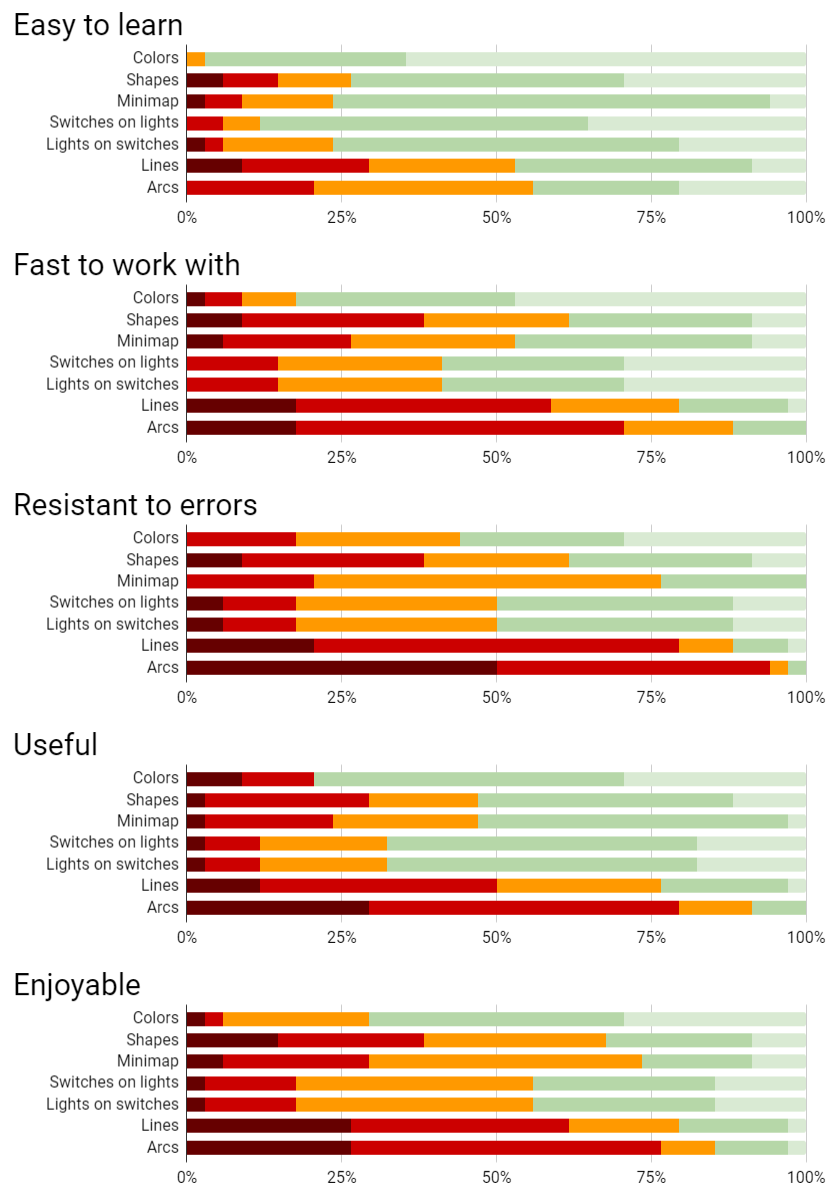
\includegraphics[width=1.0\linewidth]{exploration/results.png}
    \caption{Results of the five.}
    \label{fig:explor:lights_on_switches_vis}
\end{figure}